%%%%%%%%%%%%%%%%%%%%%%%%%%%%%%%%%%%%%%%%%%%%%%%%%%%%%%%%%%%%%%%%%%%%%%%%%%%%%%%
% \subsection{Introduction}
%%%%%%%%%%%%%%%%%%%%%%%%%%%%%%%%%%%%%%%%%%%%%%%%%%%%%%%%%%%%%%%%%%%%%%%%%%%%%%%
% \begin{frame}
%  \begin{colorblock}{blue}{lightblue}{ }
%     \Large \textbf{Introduction}
%   \end{colorblock}
% \end{frame}

\begin{frame}
\frametitle{Overview of the Lecture}
\begin{itemize}
	\item {\bf General overview of cluster scheduling principles}
	\begin{itemize}
		\item General objectives
		\item A taxonomy
		\item Current architectures
	\end{itemize}

\vspace{20pt}
	
	\item {\bf In depth presentation of three representative examples}
	\begin{itemize}
		\item Yarn
		\item Mesos
		\item Borg (Kubernetes)
	\end{itemize}
\end{itemize}
\end{frame}

%%%%%%%%%%%%%%%%%%%%%%%%%%%%%%%%%%%%%%%%%%%%%%%%%%%%%%%%%%%%%%%%%%%%%%%%%%%%%%%
\subsection{Cluster Scheduling Principles}
%%%%%%%%%%%%%%%%%%%%%%%%%%%%%%%%%%%%%%%%%%%%%%%%%%%%%%%%%%%%%%%%%%%%%%%%%%%%%%%
\begin{frame}
 \begin{colorblock}{blue}{lightblue}{ }
    \Large \textbf{Cluster Scheduling Principles}
  \end{colorblock}
\end{frame}

\begin{frame}\frametitle{Objectives}
\begin{itemize}
	\item {\bf Large-scale clusters are expensive, so it is important to use them well}
	\begin{itemize}
		\item Cluster utilization and efficiency are key indicators for good resource management and scheduling decisions
		\item Translates directly to cost arguments: better scheduling $\to$ smaller clusters
	\end{itemize}

\vspace{10pt}

	\item {\bf Multiplexing to the rescue}
	\begin{itemize}
		\item Multiple, heterogeneous mixes of application run conccurently
		\item[$\to$] The scheduling problem is a challenge
	\end{itemize}

\vspace{10pt}

	\item {\bf Scalability bottlenecks}
	\begin{itemize}
		\item Cluster and workload sizes keep growing
		\item Scheduling complexity roughly proportional to cluster size
		\item[$\to$] Schedulers must be scalable
	\end{itemize}
\end{itemize}
\end{frame}

\begin{frame}\frametitle{Current Scheduler Architectures}
\begin{figure}[h]
  \centering
  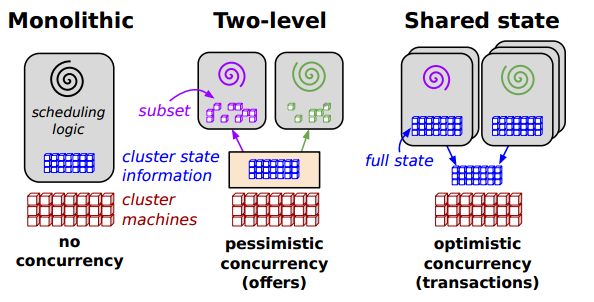
\includegraphics[scale=0.3]{./figures/intro_arch}
  \label{fig:intro_arch}
\end{figure}
\begin{itemize}
	\item {\bf Monolitic:} use a centralized scheduling and resource management algorithm for all jobs
	\begin{itemize}
		\item Difficult to add new scheduling policies
		\item Do not scale well to large cluster sizes
	\end{itemize}
	
\vspace{10pt}

	\item {\bf Two-level:} single resource manager that grants resources to independent ``framework schedulers''
	\begin{itemize}
		\item Flexibility in accommodating multiple applications
		\item Resource management and locking are conservative, which can hurt cluster utilization and performance
	\end{itemize}
\end{itemize}
\end{frame}

\begin{frame}\frametitle{Typical workloads to support}
\begin{itemize}
	\item {\bf Cluster scheduler must support heterogeneous workloads and clusters}
	\begin{itemize}
		\item Clusters are made of several generations of machines
		\item Workloads evolve in time, and can be made of a variety of applications
	\end{itemize}

\vspace{10pt}

	\item {\bf Rough categorization of job types}
	\begin{itemize}
		\item Batch jobs: e.g., MapReduce computations
		\item Service jobs: e.g., end-user facing web service
	\end{itemize}

\vspace{10pt}

	\item {\bf Knowing your workload is fundamental!}
	\begin{itemize}
		\item Next, some examples from real cluster traces
		\item The rationale: measurements can inform scheduling design
	\end{itemize}
\end{itemize}
\end{frame}

\begin{frame}\frametitle{Real cluster trace: workload characteristics}
\begin{figure}[h]
  \centering
  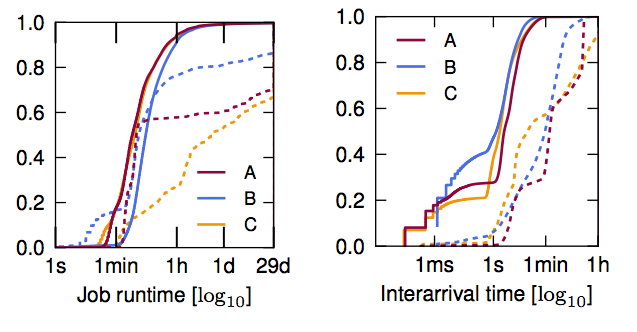
\includegraphics[scale=0.4]{./figures/intro_trace1}
  \label{fig:intro_trace1}
\end{figure}
\begin{itemize}
	\item Solid lines: batch jobs, dashed lines: service jobs
\end{itemize}
\end{frame}

\begin{frame}\frametitle{Real cluster trace: workload characteristics}
\begin{figure}[h]
  \centering
  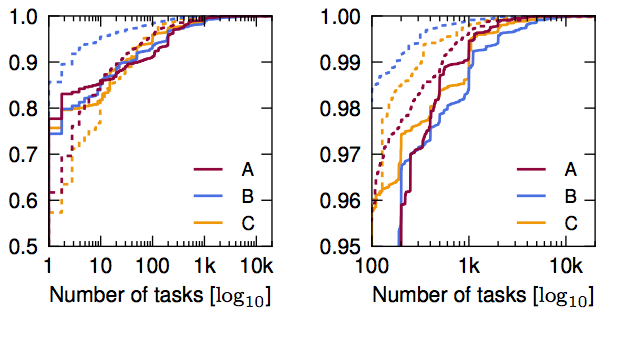
\includegraphics[scale=0.4]{./figures/intro_trace2}
  \label{fig:intro_trace2}
\end{figure}
\begin{itemize}
	\item Solid lines: batch jobs, dashed lines: service jobs
\end{itemize}
\end{frame}

\begin{frame}\frametitle{A Taxonomy}

\end{frame}


\begin{frame}\frametitle{A Taxonomy}

\end{frame}

\begin{frame}\frametitle{Architecture Details}

\end{frame}
